\chapter*{Přílohy}

% \section*{}
\addcontentsline{toc}{chapter}{Přílohy}

\begin{figure}[htbp]
    \centering
    % 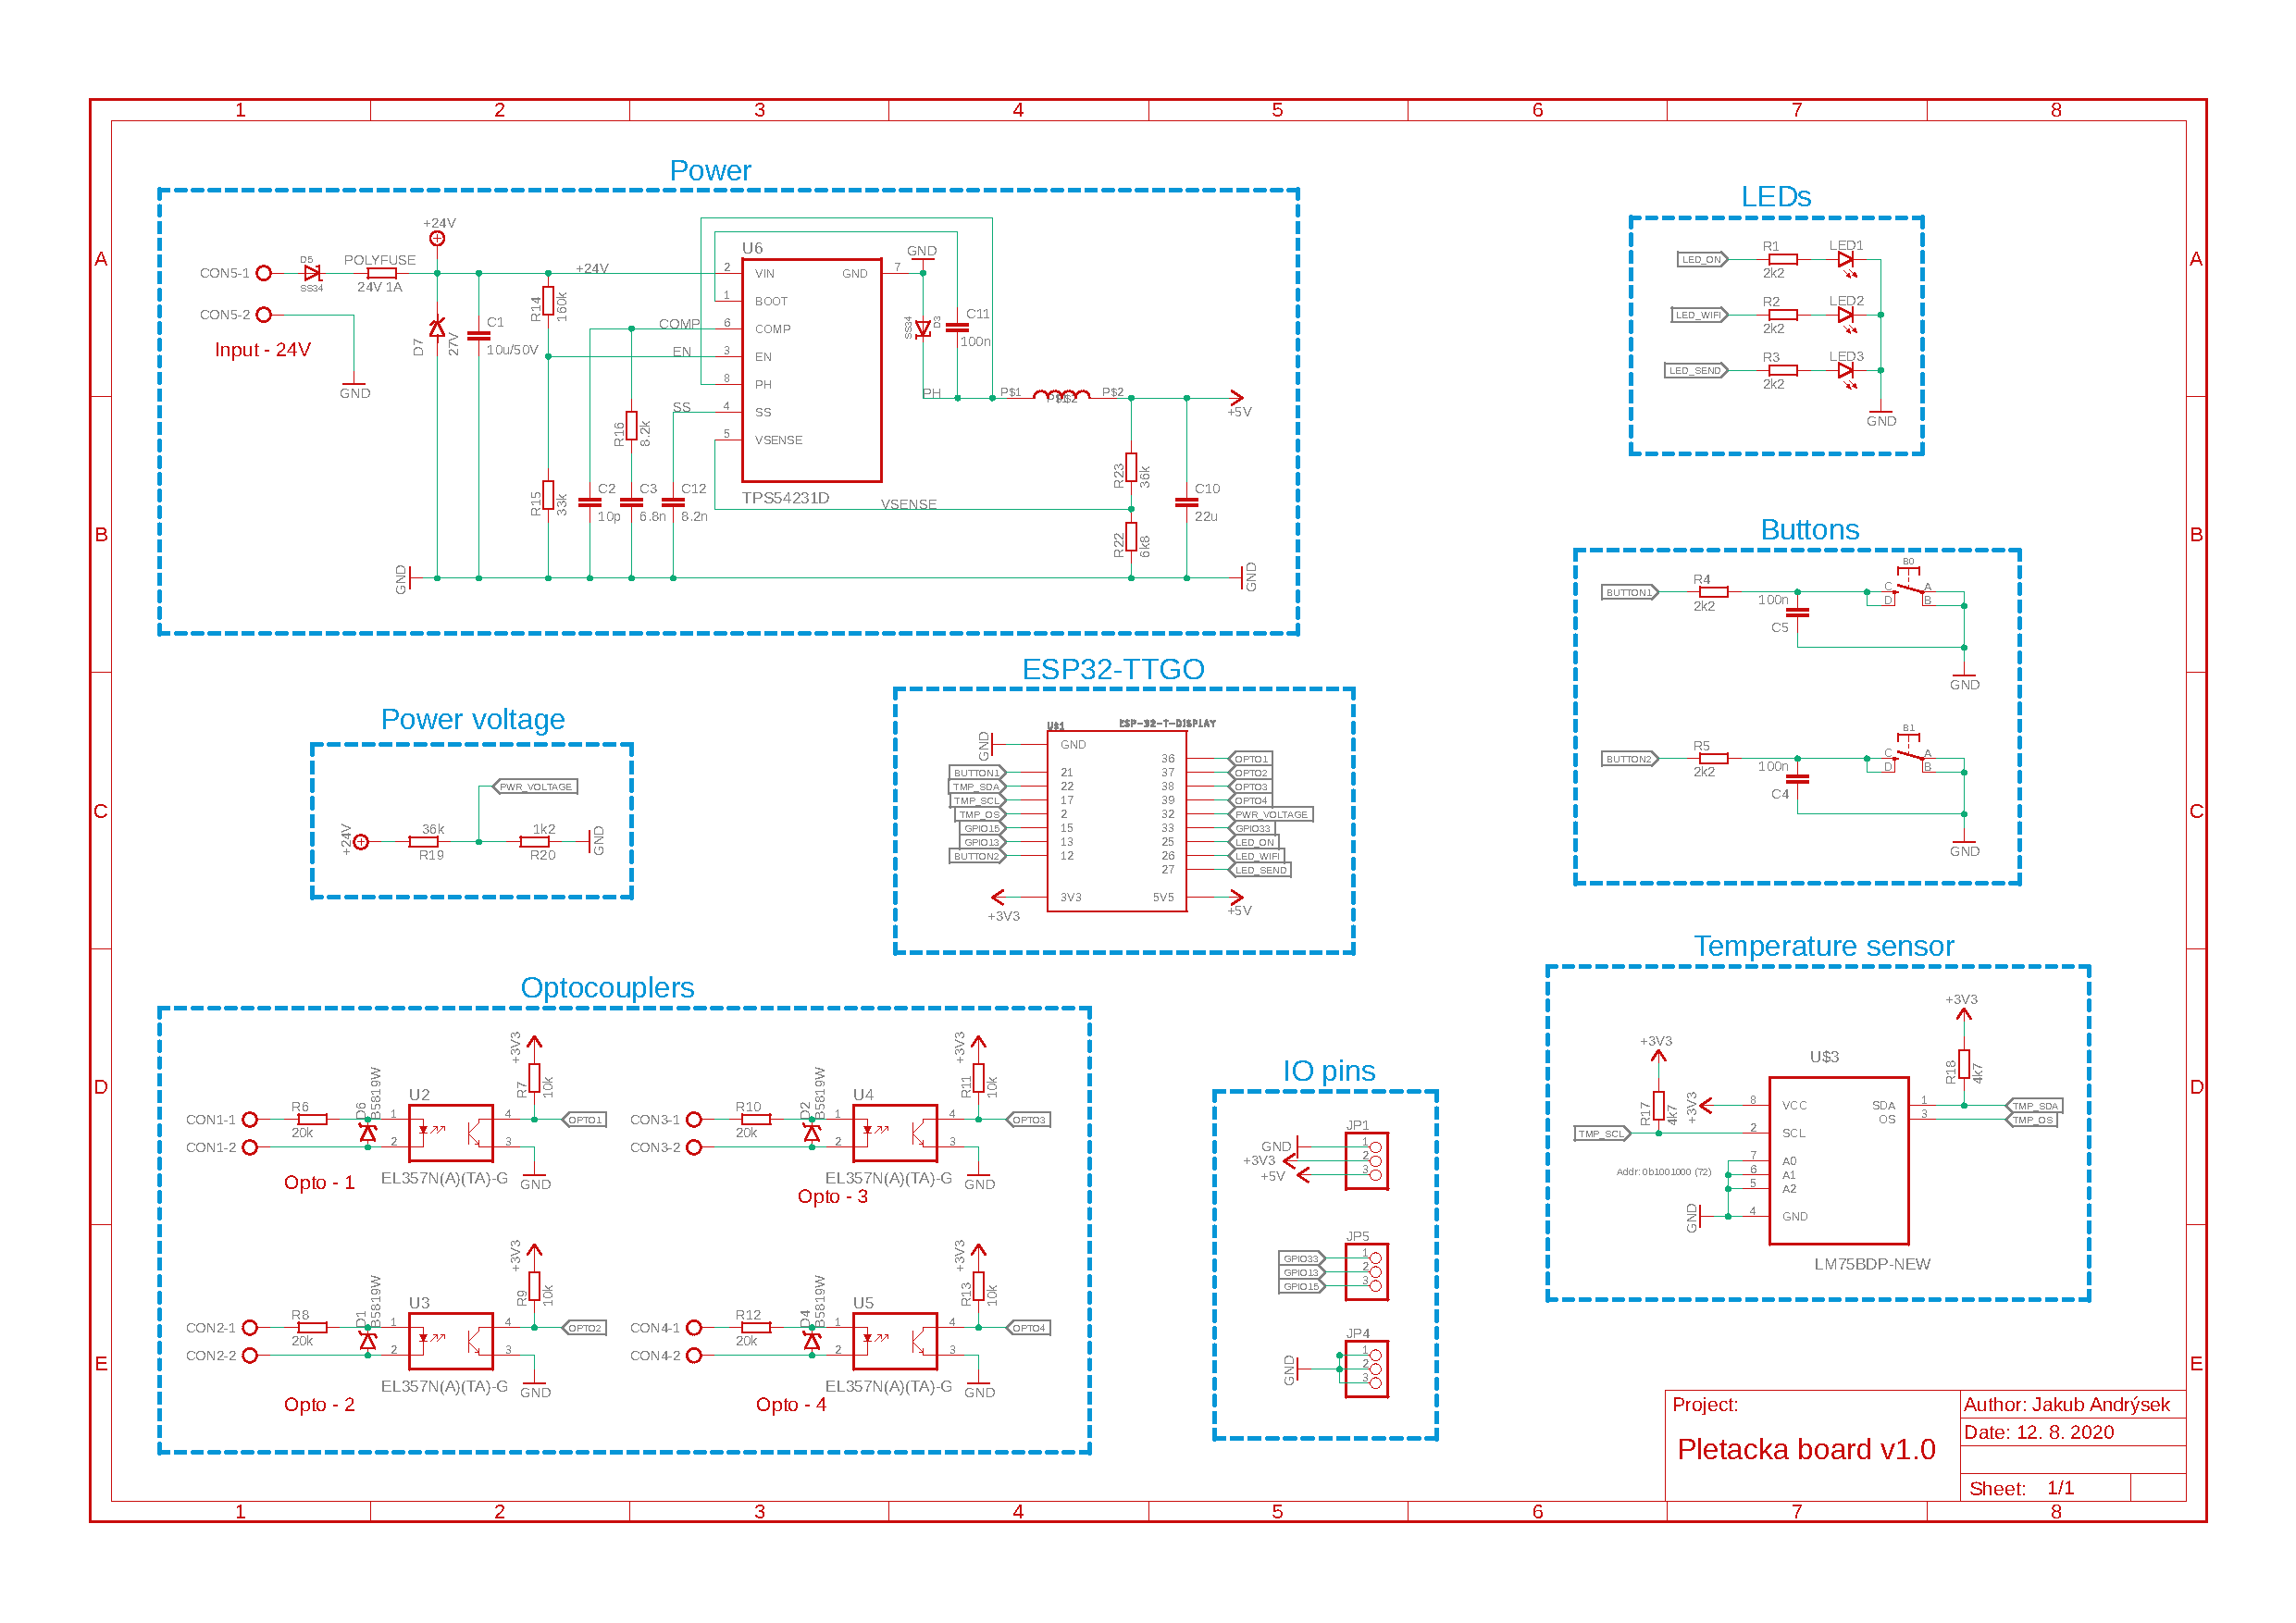
\includegraphics[scale=0.3]{DATASHEET/Pletacka_board_v1.pdf}
    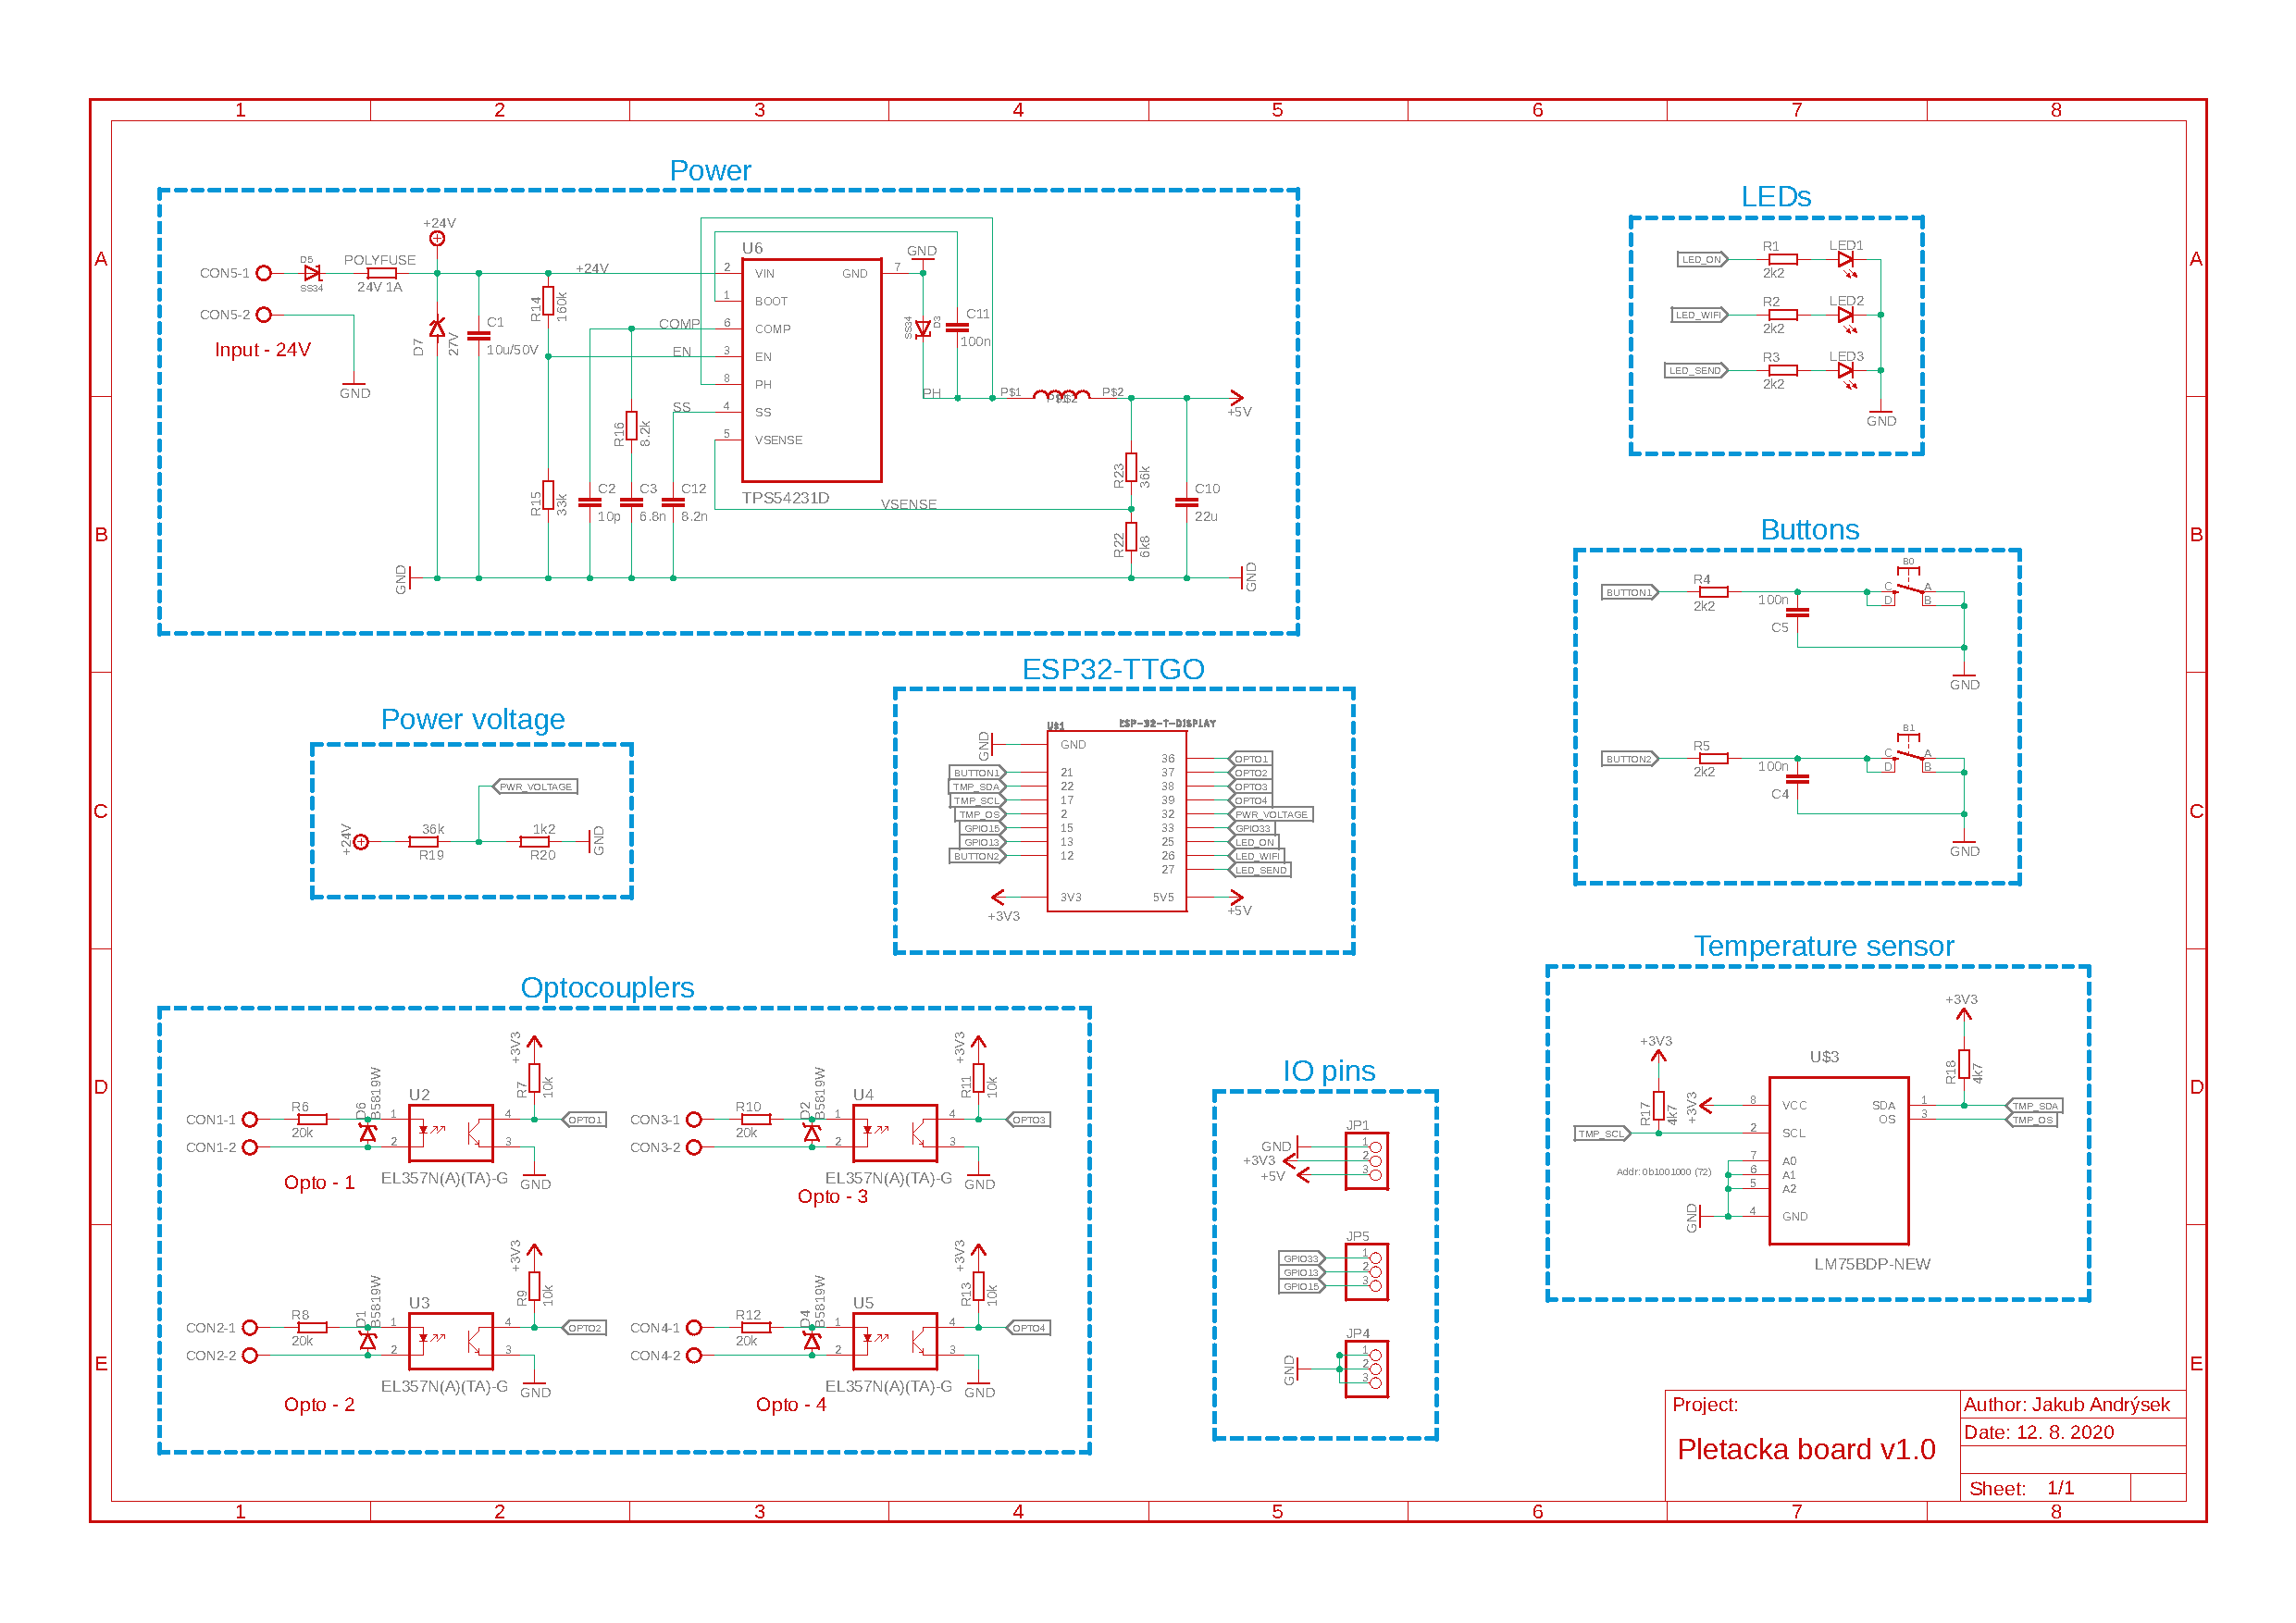
\includegraphics[width=\textwidth]{DATASHEET/Pletacka_board_v1.pdf}
    \caption{Schéma senzoru 1. verze}
    \label{fig:Schemav1}
\end{figure}


\begin{figure}[htbp]
    \centering
    % 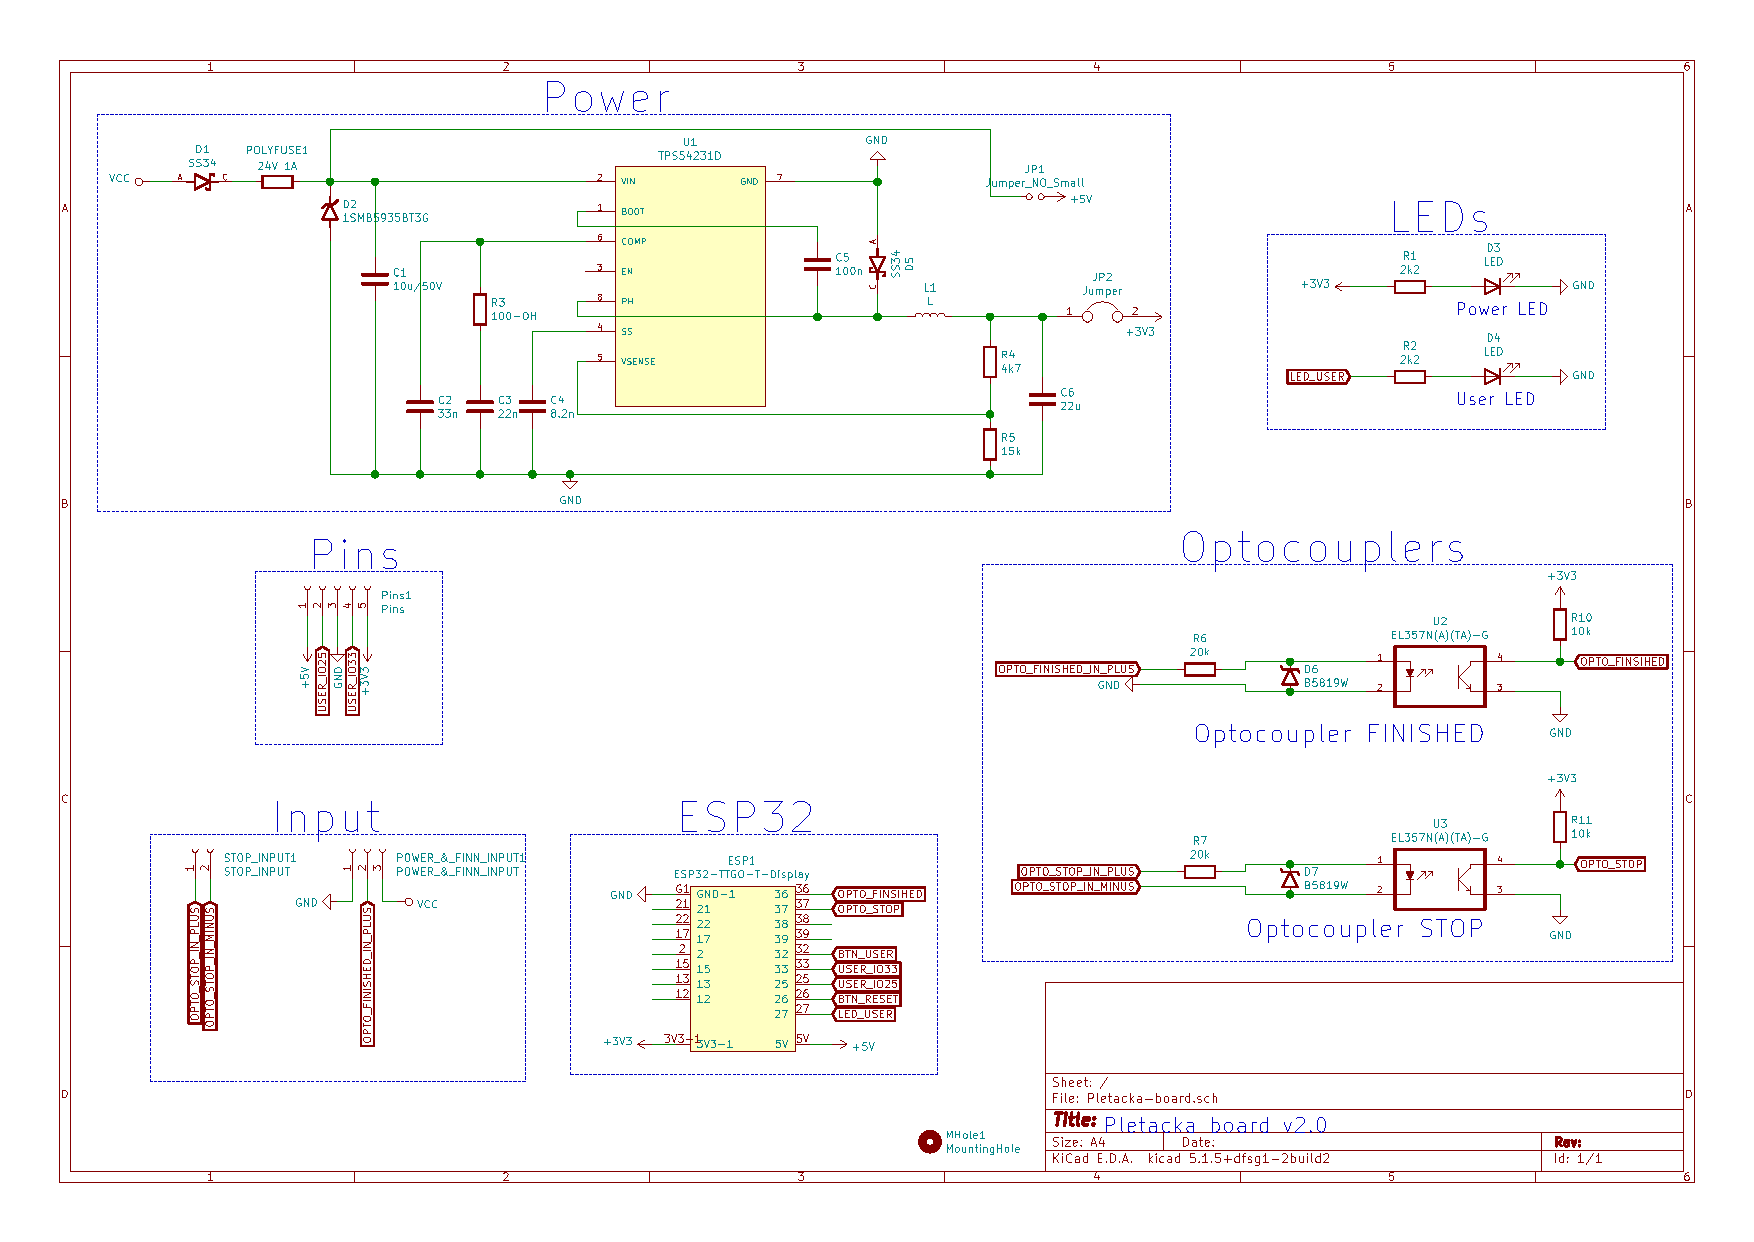
\includegraphics[scale=0.5]{DATASHEET/Pletacka_board_v2.pdf}
    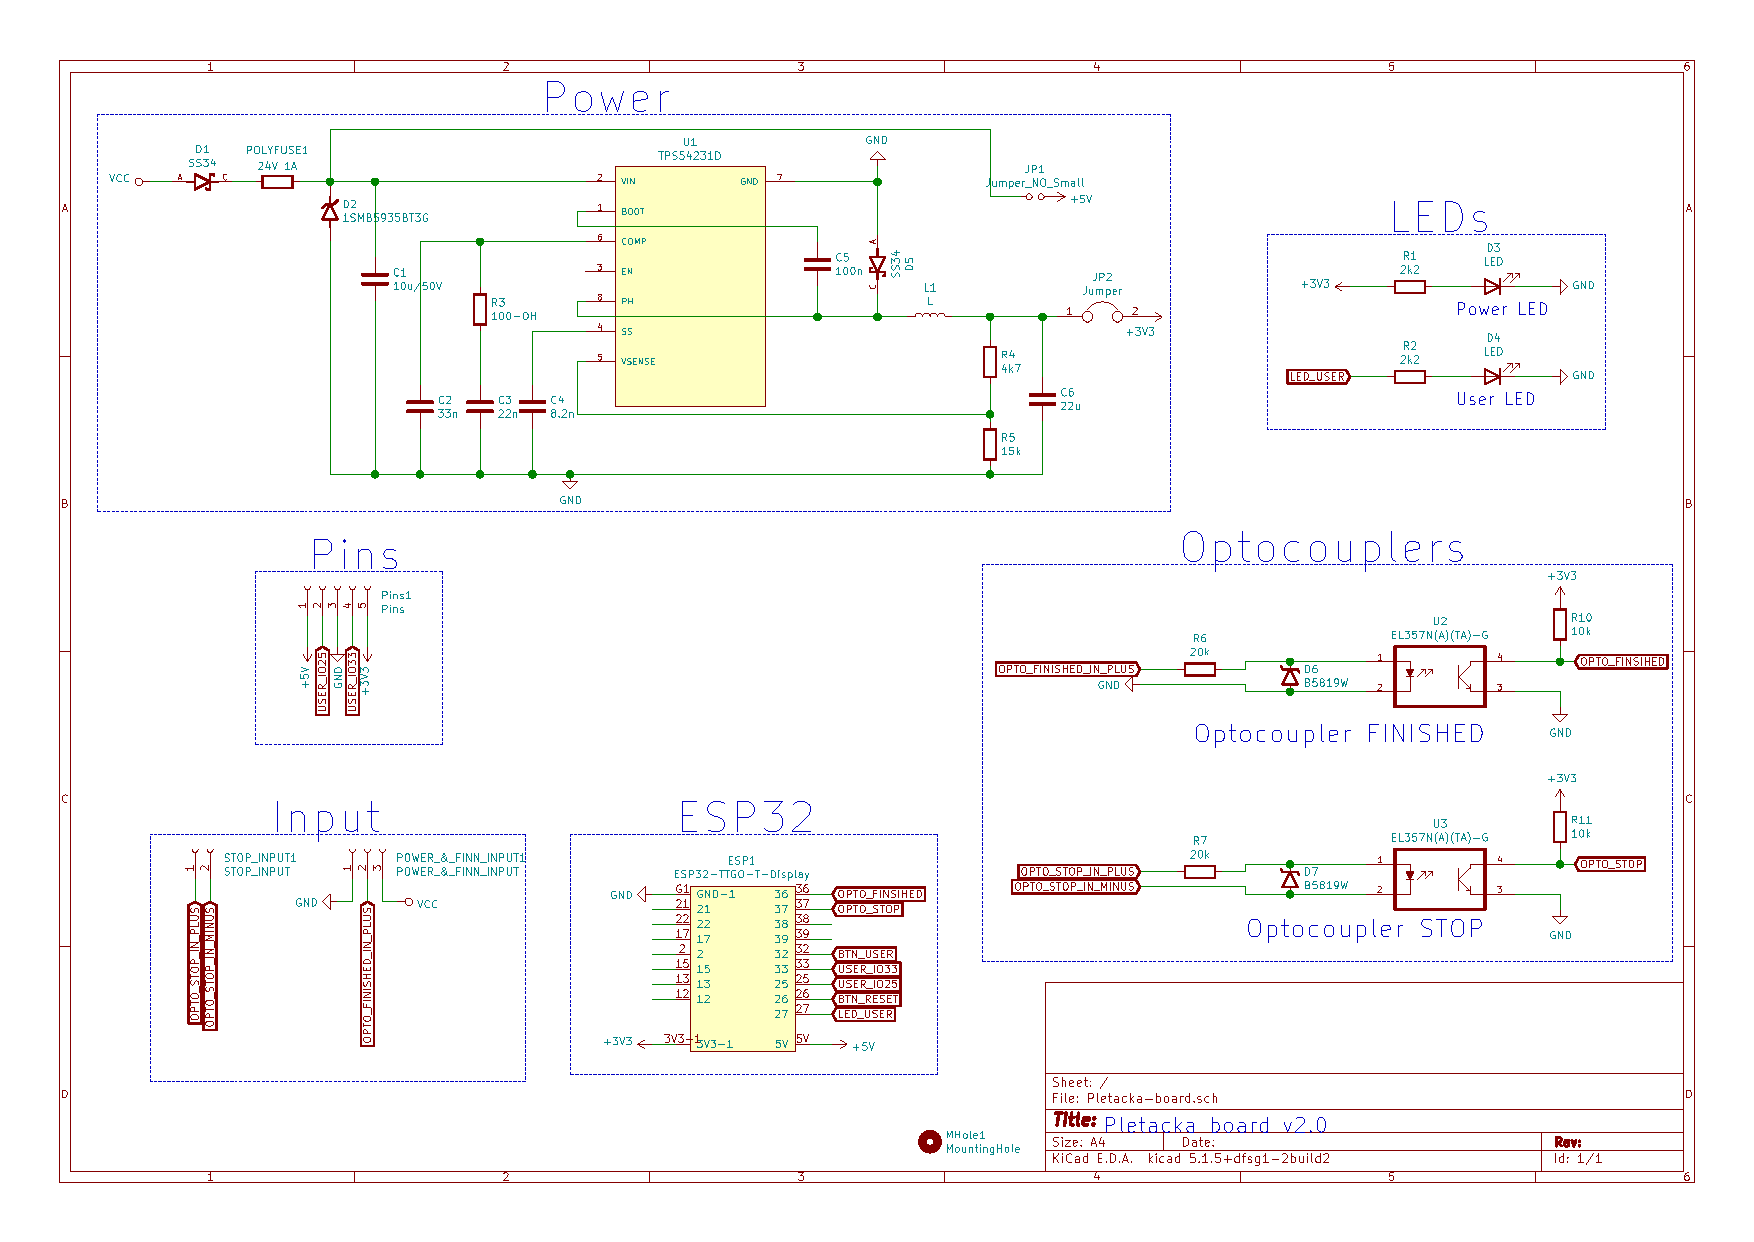
\includegraphics[width=\textwidth]{DATASHEET/Pletacka_board_v2.pdf}
    \caption{Schéma senzoru 2. verze}
    \label{fig:Schemav1}
\end{figure}

\begin{figure}[htbp]
    \centering
    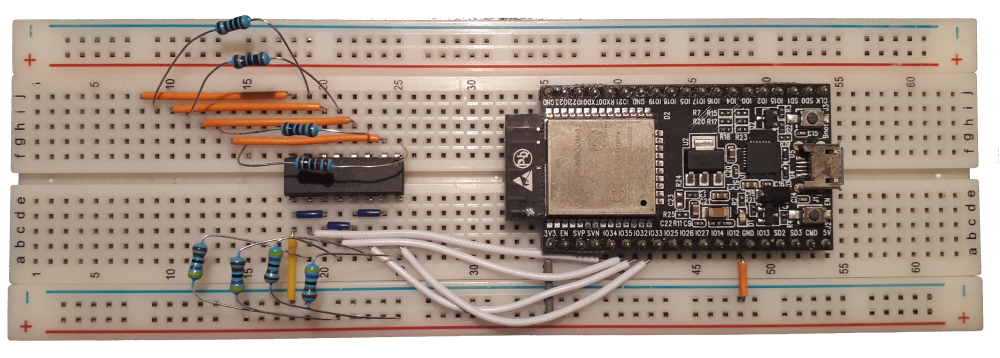
\includegraphics[width=\textwidth]{img/nepajivePole.png}
    \caption{Testování funkčnosti zapojení}
    \label{fig:Pletarna}
\end{figure}


\begin{figure}[htbp]
    \centering
    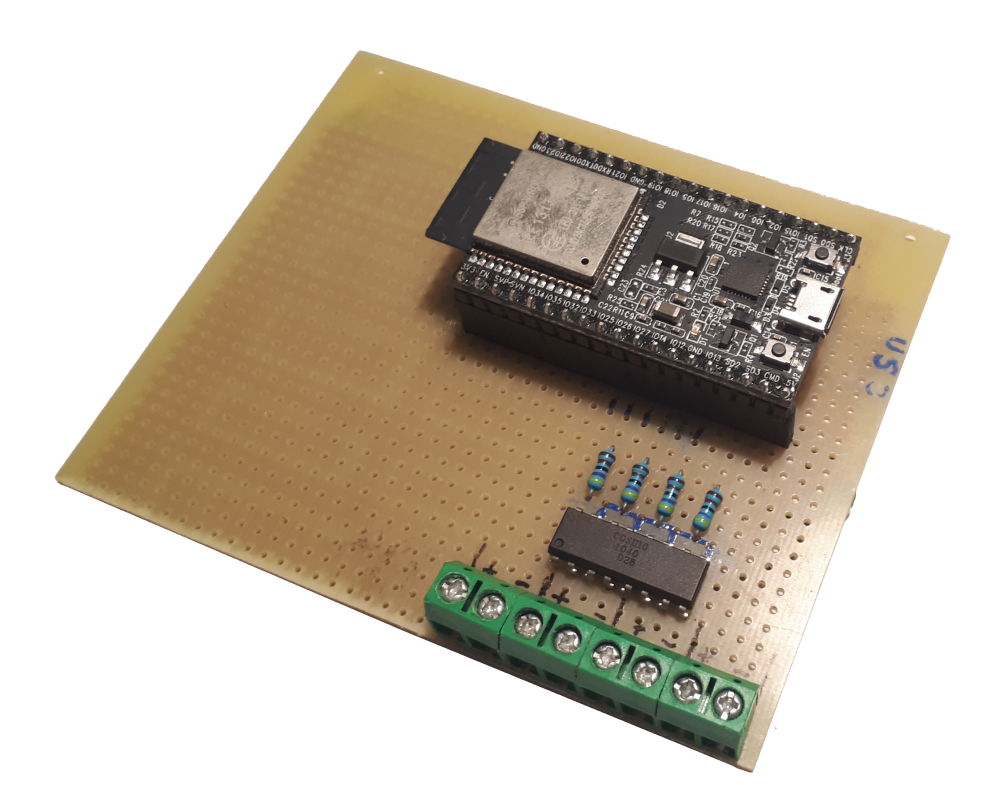
\includegraphics[width=0.8\textwidth]{img/testovaciSenzor.png}
    \caption{Testovací verze senzoru}
    \label{fig:testovaciSenzor}
\end{figure}


\begin{figure}[htbp]
    \centering
    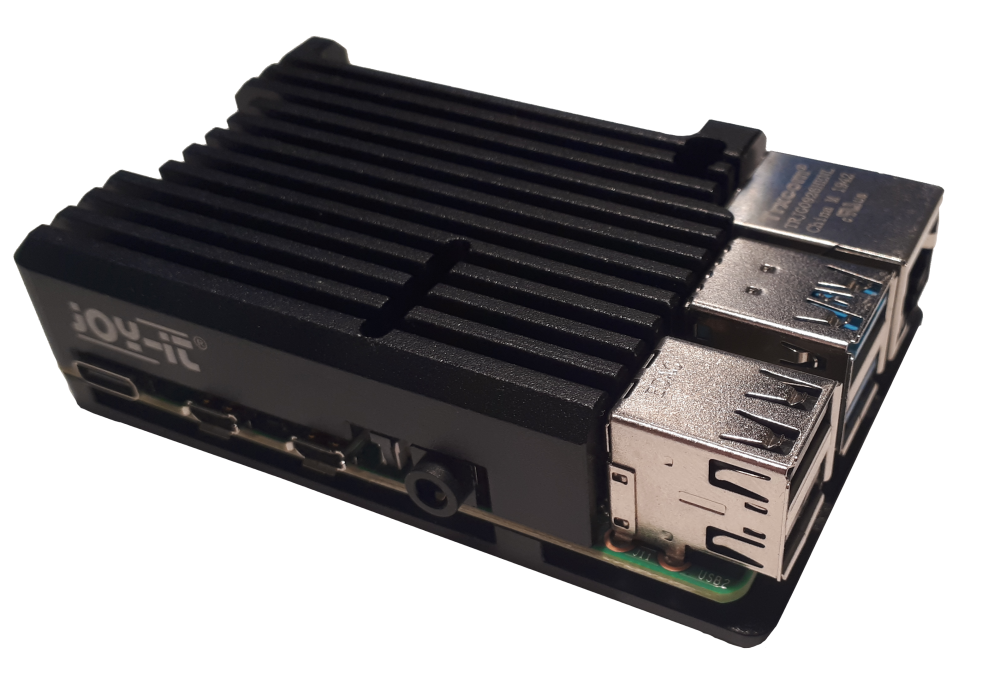
\includegraphics[width=0.8\textwidth]{img/malina.png}
    \caption{Webový server Raspberry Pi}
    \label{fig:malina}
\end{figure}


\begin{figure}[htbp]
    \centering
    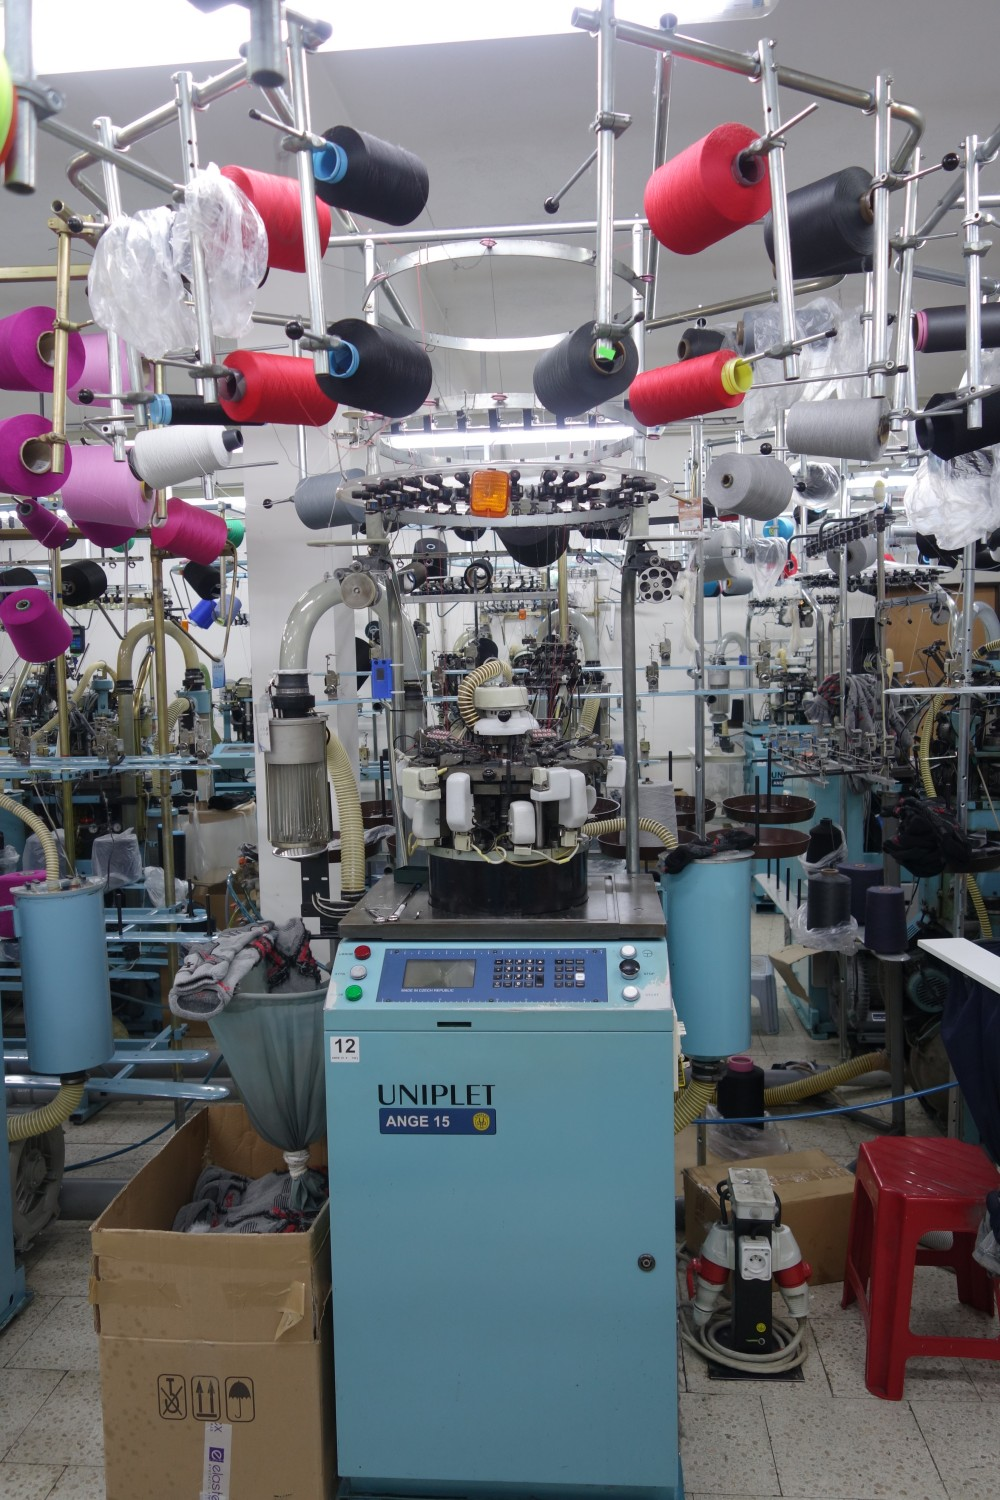
\includegraphics[width=0.9\textwidth]{img/pletacka.png}
    \caption{Pletací stroj}
    \label{fig:pletacka}
\end{figure}

\newpage